\documentclass[aspectratio=169,10pt]{beamer}
\usetheme{default}\usecolortheme{seagull}
\setbeamertemplate{navigation symbols}{}
\setbeamertemplate{footline}{\hfill{\scriptsize\color{muted}\insertframenumber/\inserttotalframenumber}\hspace{0.4cm}\vspace{0.2cm}}
\setbeamertemplate{itemize items}{\textendash}
\setbeamertemplate{enumerate items}[default]
\usepackage{fontspec}\setmainfont{TeX Gyre Pagella}\setsansfont{TeX Gyre Heros}\usefonttheme{serif}
\usepackage{booktabs,xcolor,array,graphicx,amsmath}
\setlength{\tabcolsep}{4pt}
\definecolor{ink}{HTML}{1F1F1F}\definecolor{muted}{HTML}{6B6B6B}\definecolor{accent}{HTML}{8B1A1A}
\setbeamercolor{normal text}{fg=ink}\setbeamercolor{frametitle}{fg=ink}\setbeamercolor{title}{fg=ink}
\setbeamerfont{frametitle}{size=\large,series=\bfseries}\setbeamerfont{title}{size=\LARGE,series=\bfseries}
\setbeamersize{text margin left=0.9cm,text margin right=0.9cm}
\newcommand{\muted}[1]{{\color{muted}#1}}
\newcommand{\acc}[1]{{\color{accent}#1}}
\title{Edad de exposición a la violencia y resultados adultos}
\subtitle{El fin de la violencia paramilitar en Colombia como experimento natural}
\author{Propuesta de job market paper}
\date{\muted{octubre 2026}}
\begin{document}
\begin{frame}[plain]\titlepage\end{frame}

%% 1
\begin{frame}{La pregunta}
\large ¿Depende el efecto de un shock de primera infancia de la edad a la que se recibe?
\vspace{0.8em}
\normalsize
\begin{itemize}
\item Hay periodos sensibles: el mismo shock recibido a los 0--2 años, a los 3--5 o en edad escolar deja huellas distintas en capital humano (Almond y Currie 2011; Carneiro, Salvanes, Willage y Willén, \emph{EJ}).
\item La violencia es el shock de estrés más extendido del mundo en desarrollo, y la evidencia de largo plazo existe: León (2012, Perú), Duque (2024, Colombia), Akbulut-Yuksel, Tekin y Turan (2025, Alemania).
\item Lo que esa evidencia no fija es el \textbf{gradiente por edad}: ningún estudio compara 0--2 con 3--5 y con edad escolar usando un episodio con \emph{inicio y fin fechados} y localizando al niño \emph{antes} del shock. La réplica de León (Huaroto, Gonzales y Pacheco, \emph{JHR} 2026) muestra lo que ocurre cuando no se hace: efectos antes de la concepción.
\end{itemize}
\vspace{0.6em}
\textbf{Este paper:} estima el efecto de la exposición a la violencia paramilitar por edad (in utero, 0--2, 3--5, 6--11) sobre la escolaridad y el empleo adultos, para niños nacidos en municipios en los que esa violencia \emph{terminó} en una fecha conocida.
\end{frame}

%% 2
\begin{frame}{Por qué Colombia: una violencia con actor y con fin fechado}
\begin{columns}[T]
\column{0.62\textwidth}
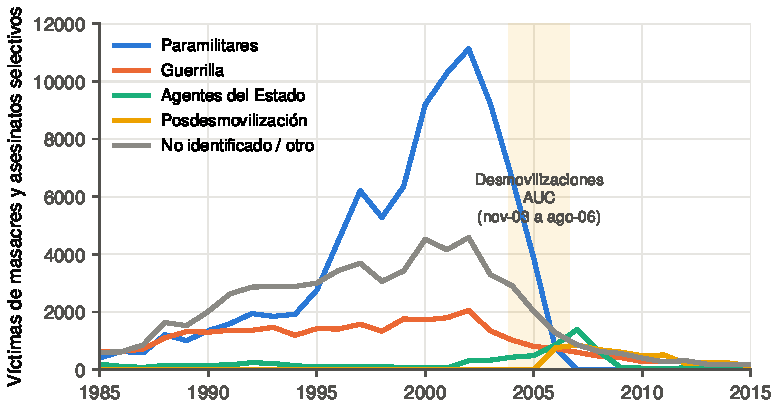
\includegraphics[width=\textwidth]{fig1_victimas_anuales.pdf}
\column{0.36\textwidth}
\small
\begin{itemize}
\item Expansión paramilitar (AUC) 1997--2002; pico 2001--02.
\item Alto el fuego en diciembre de 2002; desmovilización de los 38 bloques entre noviembre de 2003 y agosto de 2006.
\item Las víctimas paramilitares caen a cero en 2007: el fin es real, no administrativo.
\item La guerrilla sigue activa: el registro distingue perpetrador y permite controlar por ella.
\end{itemize}
\vspace{0.3em}
\muted{\scriptsize CNMH, Observatorio de Memoria y Conflicto (corte mar-2025): víctimas de masacres y asesinatos selectivos por perpetrador.}
\end{columns}
\end{frame}

%% 3
\begin{frame}{El fin se fecha municipio a municipio}
\begin{columns}[T]
\column{0.58\textwidth}
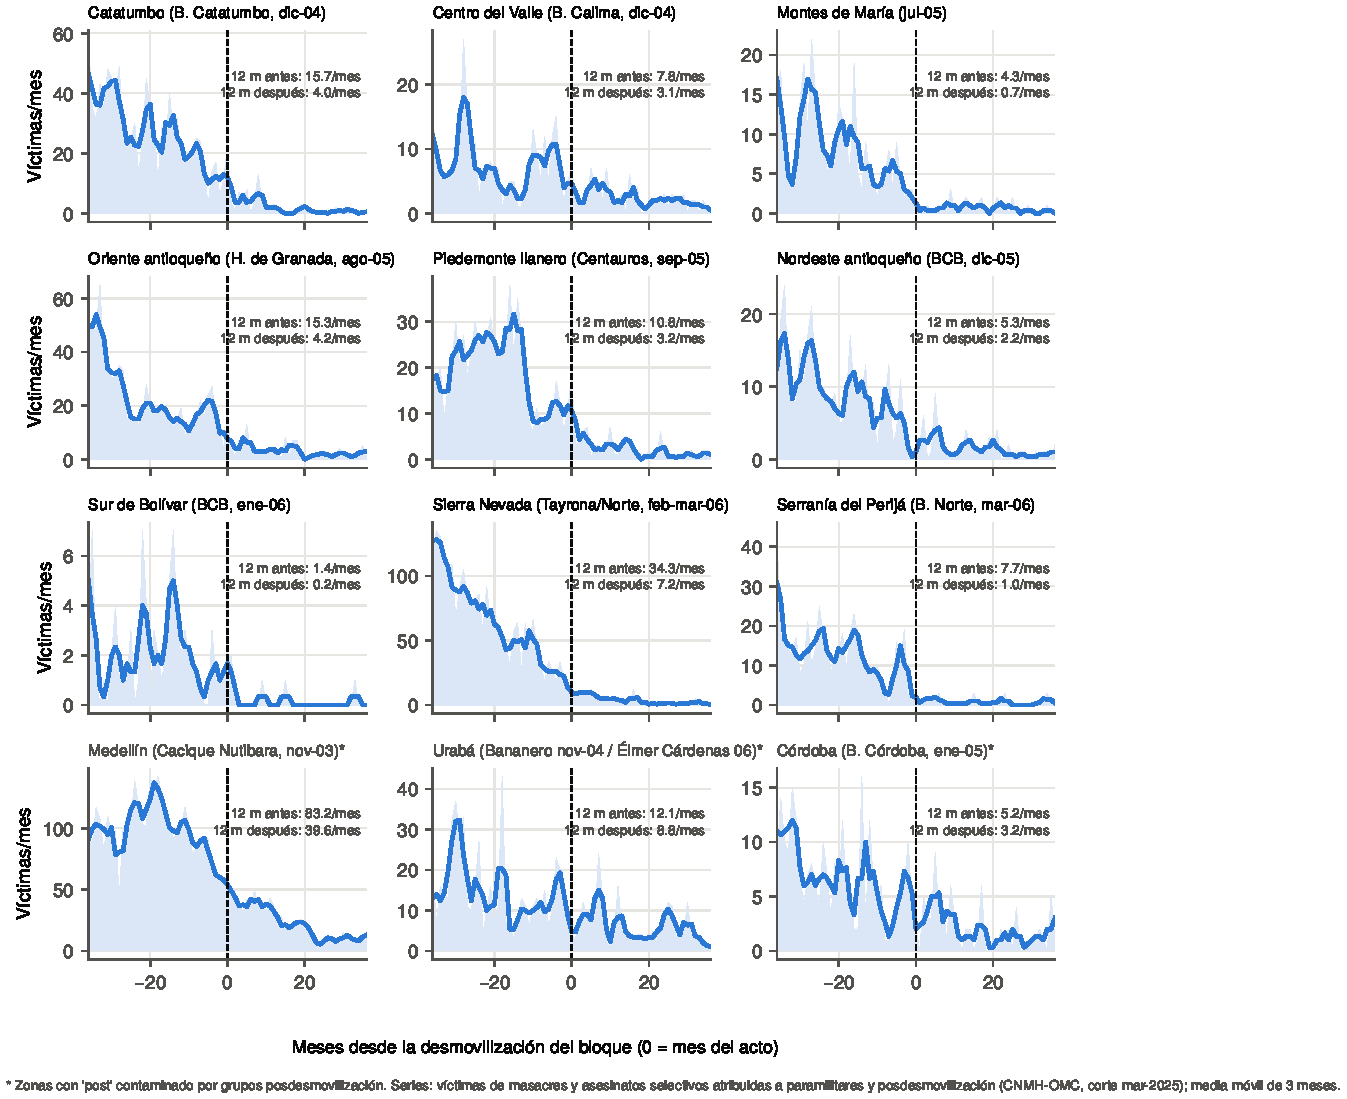
\includegraphics[height=0.72\textheight]{fig2_event_study_desmovilizacion.pdf}
\column{0.40\textwidth}
\small
\begin{itemize}
\item 451 municipios concentran el 94\,\% de las víctimas paramilitares 1997--2006; presencia mediana de 9 años.
\item Cada bloque se desmoviliza en una fecha distinta: la violencia de su zona cae en los meses anteriores y queda en cero después.
\item Para cada municipio $m$ se fecha el inicio $S_m$ y el fin $T_m$ de la presencia paramilitar (mes).
\item Lo que varía entre niños: \textbf{la edad que tenían cuando la violencia terminó en su municipio}. Un niño nacido en 2003 en Montes de María nunca la vivió; su hermano de 1998 la vivió de los 0 a los 7.
\end{itemize}
\end{columns}
\end{frame}

%% 4
\begin{frame}{El reto: la exposición no es exógena si el hogar se mueve}
\small
Colombia tiene una de las mayores migraciones internas por conflicto del mundo: en los municipios afectados, la mediana de población expulsada entre 1997 y 2010 es del 23\,\% (RUV). Por tanto:
\begin{enumerate}
\item El tiempo de exposición de un niño depende de si su hogar se queda y de a qué edad se va.
\item Irse es otro tratamiento: el hogar desplazado afronta condiciones adversas distintas de la violencia.
\item Quien se observa en el municipio años después no es quien estaba: cualquier diseño que localice al individuo en el momento del resultado mezcla el efecto con la selección.
\end{enumerate}
\vspace{0.5em}
\textbf{Cómo se resuelve aquí.}
\begin{itemize}
\item \textbf{Localización anterior al shock:} la exposición se asigna por \emph{municipio de nacimiento}, no por residencia. El estimando es intención de tratar: el efecto de nacer en un municipio donde la violencia terminará cuando el niño tenga $a$ años, con la respuesta del hogar incluida.
\item \textbf{Microdatos individuales} con municipio de nacimiento, edad en años y resultados adultos: GEIH 2012--2024 ($\sim$0,75 M personas por año; cohortes 1988--2003 observadas a los 20--36 años).
\item \textbf{La huida se mide, no se asume:} con la fecha y el motivo de la última migración (módulo de migración de la GEIH) y el registro de desplazados por municipio y año, se estima después qué parte del efecto pasa por el desplazamiento.
\end{itemize}
\end{frame}

%% 5
\begin{frame}{Especificación}
\small
Para la persona $i$, nacida en el municipio $m$ y el año $c$, observada en la encuesta del año $t$:
\begin{equation*}
Y_{imct} = \sum_{a \in \{\text{iu},\,0\text{--}2,\,3\text{--}5,\,6\text{--}11\}} \beta_a\, D^{a}_{mc} + \gamma\, \text{Post}_{mc} + \varphi\, G_{mc} + \mu_m + \lambda_{c \times d(m)} + \theta_{t} + \varepsilon_{imct}
\end{equation*}
\begin{itemize}
\item $D^{a}_{mc}$: años de presencia paramilitar en $m$ (entre $S_m$ y $T_m$) que la cohorte $c$ vivió a la edad $a$; 0 para los municipios sin presencia y para las edades posteriores a $T_m$. $\text{Post}_{mc} = 1$ si la cohorte nació después de $T_m$ en un municipio tratado.
\item $G_{mc}$: años de presencia guerrillera a las mismas edades. $\mu_m$: municipio de nacimiento. $\lambda_{c \times d(m)}$: cohorte $\times$ departamento. $\theta_t$: año de encuesta y edad al encuestar. Errores agrupados por municipio de nacimiento (451 tratados, 670 de comparación).
\item \textbf{Qué identifica $\beta_a$:} el efecto de un año de violencia paramilitar vivido a la edad $a$, comparando cohortes del mismo municipio de nacimiento que tenían edades distintas cuando la violencia terminó, neto de las tendencias de cohorte del departamento. La variación viene del calendario de $T_m$ (y de $S_m$) dentro del departamento.
\item \textbf{Resultados:} años de escolaridad, secundaria completa, educación superior, empleo, formalidad, ingreso laboral.
\end{itemize}
\end{frame}

%% 6
\begin{frame}{Qué forma del perfil distingue entre mecanismos}
\begin{center}
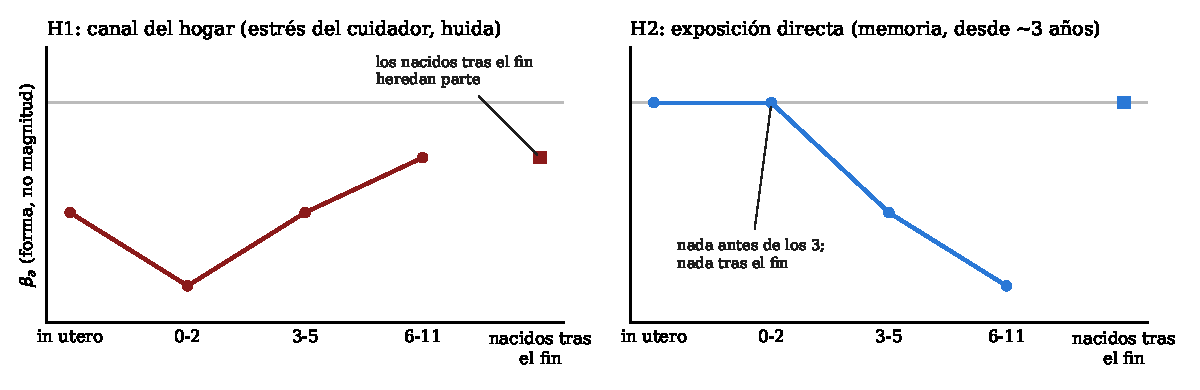
\includegraphics[width=0.9\textwidth]{fig_h1h2_min.pdf}
\end{center}
\small
\begin{itemize}
\item \textbf{H1, canal del hogar:} el daño opera a través del cuidador (estrés, huida, pérdida de ingresos): empieza in utero, es máximo a los 0--2 y los nacidos \emph{después} del fin heredan parte ($\gamma < 0$).
\item \textbf{H2, exposición directa:} el niño tiene que poder codificar la experiencia: nada antes de los 3, daño creciente con la edad, y nada para los nacidos después del fin ($\gamma = 0$).
\item Segundo paso: $\beta_a$ por separado para hogares que se desplazaron y que no (fecha y motivo de la migración en la GEIH; expulsión por municipio y año en el RUV).
\end{itemize}
\end{frame}

%% 7
\begin{frame}{Validez: qué puede fallar y cómo se comprueba}
\small
\renewcommand{\arraystretch}{1.2}
\begin{tabular}{@{}p{5.0cm}p{8.6cm}@{}}
\toprule
\textbf{Amenaza} & \textbf{Prueba} \\
\midrule
Las cohortes de los municipios tratados ya iban por otra senda & Placebo: dosis asignada a las ventanas anteriores a la concepción ($[-45,-10]$ meses) debe dar cero; cohortes 1980--87 con pendiente en la dosis futura; Rambachan y Roth (2023) \\
La violencia cambia quién nace & Nacimientos por municipio y cohorte (EEVV) sobre la dosis; composición de las madres al nacer \\
Mortalidad y emigración exterior selectivas & Defunciones por municipio y cohorte (EEVV); cotas de Lee por ventana de edad \\
Municipio de nacimiento mal medido & Cociente ocurrencia / residencia de la madre en EEVV como medida de atenuación \\
Guerrilla y fuerza pública en los mismos municipios & $G_{mc}$ y dosis de fuerza pública a las mismas edades; perfil de la guerrilla como placebo de perpetrador \\
Tratamiento continuo y escalonado & de Chaisemartin y D'Haultf\oe uille (2024); Callaway, Goodman-Bacon y Sant'Anna (2024); event study en $T_m$ \\
\bottomrule
\end{tabular}
\end{frame}

%% 8
\begin{frame}{Contribución}
\begin{enumerate}
\item \textbf{El gradiente por edad de un shock de violencia, con un episodio que termina.} Primera estimación que separa in utero, 0--2, 3--5 y 6--11 con el fin de la exposición fechado por municipio y la localización anterior al shock. El fin fechado es lo que permite el contraste limpio: cohortes del mismo municipio nacidas antes y después de que la violencia acabara.
\item \textbf{Un test de mecanismo:} canal del hogar frente a exposición directa, a partir de la forma del perfil y de los nacidos después del fin, y después por desplazamiento del hogar.
\item \textbf{Resultados adultos:} escolaridad y mercado de trabajo a los 20--36 años, no sólo puntajes en el colegio.
\end{enumerate}
\vspace{0.6em}
\small
Respecto a Duque (2024): otra década, un actor con fin fechado, municipio de nacimiento en lugar de residencia y resultados adultos. Respecto a León (2012) y su réplica: el placebo pre-concepción es parte del diseño, no una comprobación posterior.
\end{frame}

%% 9
\begin{frame}{Datos y calendario}
\small
\begin{columns}[T]
\column{0.5\textwidth}
\textbf{Datos}
\begin{itemize}
\item CNMH-OMC: víctimas por municipio, mes y perpetrador 1985--2015 (en mano; $S_m$ y $T_m$ construidos para los 451 municipios).
\item RUV: expulsados por municipio y año (en mano).
\item GEIH 2012--2024: municipio de nacimiento, migración, educación, empleo, ingreso (público; descarga pendiente).
\item EEVV nacimientos 1998--2010 y defunciones 1998--2019 (público; descarga pendiente).
\end{itemize}
\column{0.5\textwidth}
\textbf{Calendario}
\begin{itemize}
\item Meses 1--2: GEIH y EEVV; dosis por municipio de nacimiento $\times$ cohorte; conteos y potencia (criterio: MDE $\le 0{,}05$ DE en escolaridad por ventana).
\item Meses 3--5: estimación principal, placebos, perfil por desplazamiento.
\item Mes 6: borrador y decisión. Si el placebo pre-concepción falla con municipio de nacimiento, el diseño no sirve y se dice.
\item Meses 7--18: robustez, extensiones, paper completo.
\end{itemize}
\end{columns}
\end{frame}
\end{document}
